\section{Erweiterungen (Fabio Aubele)}\label{sec:erweiterungen}
Da ArtBot nur innerhalb eines Semesters geplant, implementiert und dokumentiert wurde, gibt es viele Möglichkeiten, wie das Projekt zusätzlich ergänzt werden kann. Innerhalb dieses Abschnittes soll dabei zunächst auf mögliche Verbesserungen und zusätzliche Funktionen der Anwendung eingegangen werden. Daraufhin wird eine Anleitung geschildert, mit dessen Hilfe der Chatbot um weitere Logik ergänzt werden kann.

\subsection{Verbesserungen und zusätzliche Funktionalitäten}
Die entwickelte Anwendung kann mit vielen Verbesserungen ergänzt werden. Zunächst wäre die generelle Architektur der 'custom-actions' zu nennen. Momentan gibt es für jeden der drei Gesprächsfälle aus Kapitel \ref{sec:dialog} eine 'custom-action'. Diese holt sich anhand der Eingabe vom Benutzer die Informationen aus der Datenbank. Je nachdem welche und wie viele Daten zurückgegeben wurde, was wiederum signalisiert, ob die Eingabe des Benutzers korrekt war, wird eine Ausgabe des Chatbots ausgelöst. Eine weitaus sauberere Möglichkeit wäre es jedoch, für jeden Fall zwei 'custom-actions' zu implementieren. Die erste holt sich die Daten aus der Datenbank und die zweite kümmert sich um die Ausgabe. Somit wäre mehr Rücksicht auf das Prinzip 'Separation of Concerns' genommen, was zur Übersicht und Qualität des Codes beitragen würde.\\
\\
Eine der wichtigsten Verbesserungen wäre das Hinzufügen von Small-Talk. Dies würde erlauben, dass der Chatbot auf ganz alltägliche Kommunikationen mit der richtigen Antwort reagieren kann. Dies kann folgende Fragen miteinbeziehen: "Wie geht es dir?", "Wie ist das Wetter heute?", "Wo kommst du her\shorthandoff{"}?" oder \shorthandon{"}"Bist du ein Mensch?". Wichtig dabei ist, dass der Chatbot mit der richtigen Strategie antwortet. Hierbei sollte der Bot also immer auf das Thema Künstler und Kunstwerke hinleiten, dies allerdings nie so abrupt, dass der Benutzer sich übergangen fühlt. Für diese Ergänzungen kann auch die Anleitung unter Kapitel \ref{sec:logik} dienen.\\
\\
Eine weitere Verbesserung würde das Hinzufügen von Stemming und Lemmatization erlauben. Stemming ermöglicht es einzelne Wörter auf ihren Stamm zu reduzieren. Hierdurch wird erreicht, dass verschiedene Formen des selben Wortes nur durch einen Stamm dargestellt werden \cite{stemming}, wie in Abbildung \ref{stemm} mit einem englischen Wortbeispiel zu sehen ist.
\begin{figure}[htbp]
	\centerline{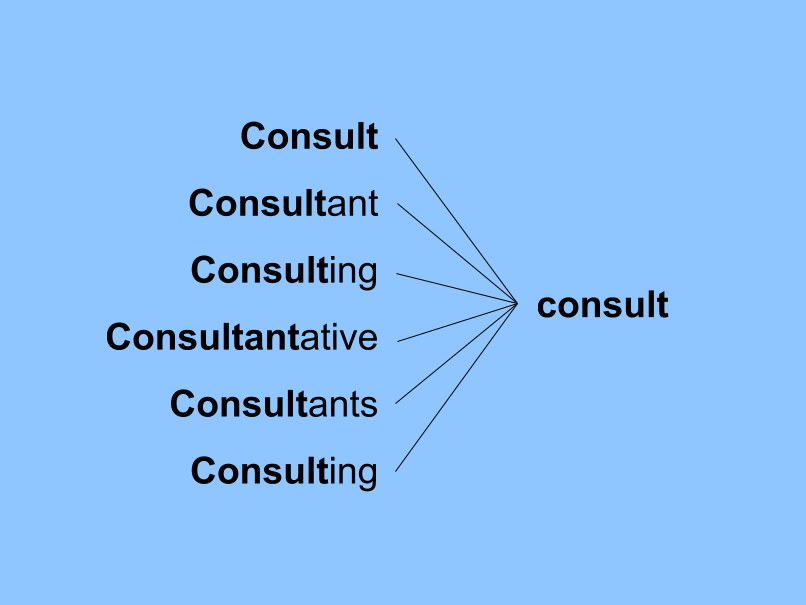
\includegraphics[width=0.5\linewidth]{figures/stemm.png}}
	\caption{Stemming des englischen Wortes 'consult' \cite{stemming2}.}
	\label{stemm}
\end{figure}
Dem entwickelten Chatbot würde dies ermöglichen, auch Eingaben des Nutzers zu verstehen, welche eventuell falsch geschrieben worden sind \cite{stemming}. Innerhalb der entwickelten Anwendung ArtBot müssten die Trainingsdaten, welche die Eingaben des Benutzers widerspiegeln und für Rasa NLU verwendet werden, mithilfe von Stemming abgeändert werden. Daraufhin müsste das neuronale Netz mit den neuen Daten trainiert werden. Dadurch wäre die Erkennung der Eingaben deutlich robuster und zusätzlich wird Redundanz bei der Formulierung der Trainingsdaten verhindert \cite{stemming}.\\
Lemmatization erweitert den eben geschilderten Grundgedanken von Stemming, dabei gilt es nicht nur den Wortstamm zu finden, sondern die wirkliche Normalform des Wortes \cite{stemming}, hier ein Beispiel für ein konjugiertes Verb:\\
sehen, siehst, sah,... -> Normalform: sehen\\
Dies würde dem Chatbot helfen, auch Sätze welche womöglich konjugiert worden sind, korrekt zu erkennen. Zur Umsetzung kann das nltk-Paket\footnote{siehe \href{https://www.nltk.org/}{https://www.nltk.org/}} (Natural Language Tool Kit) in Python benutzt werden, eine Anleitung dafür bietet Referenz \cite{stemming}.\\
\\
Um die Qualität des Chatbots zu erweitern, könnte eine zusätzliche KI-Komponente entwickelt werden. Hier wäre es möglich, das Gespräch mit dem Benutzer genauer zu analysieren. Hat es der Nutzer hierbei nicht innerhalb von ca. 10 Eingaben geschafft, ein Bild auszugeben (Hauptfunktion des Bots) kann eine zusätzliche Ausgabe angezeigt werden, welche die Funktion und die gewünschten Eingaben genau erklärt.\\
Zusätzlich wäre es eine Verbesserung, die Gespräche von ArtBot zu loggen und aus den Log-Dateien neue Daten abzuwandeln, mit welchen der Chatbot wiederum trainiert werden kann. Somit würde der Chatbot durch seine eigenen Konversationen lernen.\\
\\
Die letzte Ergänzung beschreibt eine aufwändigere Änderung. Jedoch wäre es möglich, den Benutzer die Antwort des Chatbots bewerten zu lassen. Dies könnte mit einem Daumen runter Daumen hoch Prinzip realisiert werden. Hierfür müsste für jede Ausgabe des Bots die Wertung des Benutzers zusätzlich mitgeloggt werden. Auch die vorhandene GUI müsste mit neuen Bedienelementen ergänzt werden. Daraufhin lässt sich anhand der erzeugten Daten analysieren, bei welchen Eingaben der Bot eventuell Schwächen aufweist und wo Verbesserungspotenzial besteht.

\subsection{Erweitern der Chatbot-Logik}\label{sec:logik}
Nun soll beschrieben werden, wie die Chatbot-Logik ergänzt werden kann. Zuerst ist zu erwähnen, dass es prinzipiell immer möglich ist, für die momentan bestehenden Gesprächsfälle mehr Vorlagen als Trainingsdaten zu erstellen. Dies würde erlauben, dass auch bei sehr unterschiedlichen Formulierungen des Benutzers die selben Ausgaben zur Verfügung stehen und somit der Chatbot eine konstant bessere Leistung aufzeigt. Innerhalb dieses Kapitels soll jedoch hauptsächlich erklärt werden, wie es möglich ist die Logik des Chatbots zu ergänzen und somit zu erlauben, dass der Bot auch auf andere Gesprächsfälle Bezug nimmt.\\
Hierbei müssen zwei Fälle unterschieden werden. Der erste betrifft Änderungen, welche nur auf eine einfache textuelle Ausgabe des Bots abzielen und der zweite Fall ist für Änderungen, welche externe Logik benötigen. Innerhalb von ArtBot werden dabei meist immer Informationen aus der Datenbank benötigt.\\
\\
Für den ersten Fall muss zunächst ein neuer Intent angelegt werden, welches die potenziellen Eingaben des Nutzers auflistet. Ebenfalls muss der Intent innerhalb einer Story vorkommen mit der entsprechenden Antwort des Bots. Die genaue Syntax des Intents und der Story ist in der Seminararbeit in Quelle \cite[S.10]{seminar} genauer beschrieben. Nun muss noch die Antwort des Chatbots definiert werden. Dies geschieht innerhalb der Domain-Datei (\textit{domain.yml}), wie in Code \ref{domain} zu sehen ist.
\begin{lstlisting}[caption={Einfügen einer neuen Antwort des Chatbots.}, label=domain, lineskip=1pt,
morekeywords={actions, templates, text}]
actions:
  - utter_goodbye
...
templates:
  utter_goodbye:
    - text: Auf Wiedersehen!
    - text: Machs gut!
    - text: Bis bald!
...
\end{lstlisting}
Hierbei muss unter \texttt{actions} nur der generelle Name aufgelistet werden, welcher bei einer textuellen Antwort der Konvention nach mit \texttt{utter\_} anfängt. Unter \texttt{templates} muss dann für jede Antwort der auszugebende Text angegeben werden. Bei mehreren Angaben wird eine zufällig ausgewählt, was bei häufig vorkommende Antworten für mehr Vielfalt sorgt. Wurde alles entsprechend geändert, müssen nun die neuronalen Netze neu trainiert werden, da sich die Trainingsdaten durch das Hinzufügen eines neuen Intent und einer neuen Story geändert haben. Dies geschieht mit der Eingabe \texttt{rasa train} in der Kommandozeile, welche innerhalb der Quelle \cite{command} unter 'Train a Model' genauer beschrieben ist. Daraufhin kann der Bot auf die neue Benutzer-Eingabe mit dem gewünschten Verhalten reagieren.\\
\\
Der zweite Fall benötigt mehr Änderungen. Hier muss ebenfalls ein neuer Intent und eine neue Story angelegt werden. Jedoch wird hier keine einfache textuelle Antwort des Chatbots gebraucht, sondern es wird eine neue 'custom-action' benötigt. Diese muss auch in der Domain-Datei allerdings nur unter \texttt{actions} erwähnt werden, wie in Code \ref{domain} oben zu sehen ist. Die Konvention dabei ist, dass diese mit \texttt{action\_} angeführt werden. Grundlegend wird jede 'custom-action' durch eine eigene Klasse in einer eigenen Python-Datei repräsentiert. Die grundlegende Struktur dieser Klasse und der Datei ist immer gleich. Ein Beispiel ist in Code \ref{custom} zu sehen.
\begin{lstlisting}[caption={Beispiel für den Aufbau einer 'custom-action'.}, label=custom, lineskip=1pt,showlines=true]
from rasa_sdk import Action, Tracker
from rasa_sdk.executor import CollectingDispatcher
from rasa_sdk.events import SlotSet

import database_api as api

class ActionFetchArt(Action):

  def name(self):
    return "action_fetch_art"

  def run(self, dispatcher: CollectingDispatcher, tracker: Tracker, 
          domain: Dict[Text, Any]):
    # get slots
    user_art = tracker.get_slot('art')
    # get images from database
    images = api.get_pictures_by_title(user_art)
	...
    # output a message
    dispatcher.utter_message("Hier das gewünschte Bild!")
    # set slot back to default
    return [SlotSet("art", None)]
    
\end{lstlisting}
Zunächst benötigt es einige Dateien der Bibliothek Rasa, welche importiert werden. Zusätzlich ist auch die Datenbank-API bereits importiert worden (Zeile 5). Daraufhin wird eine Klasse erstellt, welche die 'custom-action' widerspiegelt. Hierbei sind zwei Methoden Pflicht. Die erste Methode \texttt{name()} gibt lediglich den Namen der 'custom-action' zurück. Dies muss derselbe Name sein, welcher auch in der Domain-Datei und in der Story genannt ist, damit Rasa diese zuordnen kann. Die zweite Methode \texttt{run()} beinhaltet die gesamte Logik. Einige beispielhafte Schritte sind dabei aufgeführt. So wird in Zeile 15 ein Slot namens \texttt{'art'} ausgelesen. In Zeile 17 werden sich alle Kunstwerke aus der Datenbank geholt, welche den selben Namen haben, wie in der Slot angegeben wurde. Daraufhin wird in Zeile 20 eine textuelle Antwort des Chatbots ausgegeben. Abschließend wird in Zeile 22 die Slot auf den default-Wert \texttt{None} zurückgesetzt. Durch diesen return-Wert ist es möglich Slots final abzuändern, dies muss allerdings nicht angegeben werden. Die Klasse und auch die Datei kann natürlich beliebig mit zusätzlich benötigten Funktionen oder Klassen ergänzt werden.\\
\\
Die Logik von ArtBot kann mithilfe der Werte zur Epoche (z.B. Renaissance, Barock) und zur Art des Bildes (z.B. Porträt, religiös, geschichtlich), welche bereits innerhalb der Datenbank abgelegt sind, ergänzt werden. Somit wäre es durch die oben beschriebenen Schritte möglich, je nach Wunsch des Benutzers alle Kunstwerke der Renaissance anzuzeigen oder aller Bilder mit religiösen Motiven. Ebenfalls ist bereits das Geburtsdatum des Künstlers angegeben, welches durch Erweiterung der Logik des Chatbots ausgegeben werden kann, sofern der Benutzer danach fragt.
